% Sébastien Tosi (sebastien dot tosi at irbbarcelona dot org)
% BioImage Data Analysis Textbook 

\documentclass[11pt,a4paper,oneside]{report}
% Palatino for rm and math | Helvetica for ss | Courier for tt
\usepackage{mathpazo} % math & rm
\linespread{1.05}        % Palatino needs more leading (space between lines)
\usepackage[scaled]{helvet} % ss
\usepackage{courier} % tt

\normalfont
\usepackage[T1]{fontenc}
\usepackage[footnotesize]{caption}
\usepackage{subfig}

\linespread{1.05}         % Palatino needs more leading (space between lines)

% space between paragraphs
\parskip 7.2pt

%making 1.5 spaced lines
\usepackage{setspace}
\onehalfspacing

% background shading
\usepackage{framed}

\usepackage{pdfsync}

% indent
\setlength{\parindent}{0in} % avoids indent at the beginning of paragraph


%\usepackage{url} % omitted, as this will just show url in different font
\usepackage[pdftex]{graphicx}

%% Color definitions
\usepackage{color}
\definecolor{gray09}{rgb}{0.9,0.9,0.9}  %background for codes
\definecolor{red}{rgb}{1,0,0}
\definecolor{blue}{rgb}{0,0,1}
\definecolor{lightblue}{rgb}{0,0.8,1}
\definecolor{Dark}{gray}{.2}
\definecolor{Medium}{gray}{.6}
\definecolor{Light}{gray}{.8}
\definecolor{shadecolor}{rgb}{0.9, 0.9, 1}


%% enable using eps figure.
\usepackage{epstopdf}

%% Citations. 
%% Natbib is a popular style for formatting references.
\usepackage{natbib}
%% bibpunct sets the punctuation used for formatting citations.
\bibpunct{(}{)}{;}{a}{,}{,}

\usepackage{hyperref}
\hypersetup{colorlinks=true, 
    citecolor=blue, 
	linkcolor=black, 
	urlcolor=black}


%%%%%%%% Header and Footer %%%%%%%%
\usepackage{fancyhdr}
\setlength{\headheight}{15.2pt}
%\pagestyle{fancy}
\pagestyle{fancyplain}
\renewcommand{\chaptermark}[1]{\markboth{#1}{}}
\renewcommand{\sectionmark}[1]{\markright{\thesection\ #1}{}}
 
\lhead{\fancyplain{}{\textit{BIAS 2015}}}
\chead{}
\rhead{\fancyplain{}{\textit{\rightmark}}}
\lfoot{}
\cfoot{\fancyplain{}{\thepage}}
\rfoot{}


%%%%%%%% Custom Environments %%%%%%%%

%% a block for excercies
\newenvironment{indentexercise}[1]%
{{\setlength{\leftmargin}{2em}}%
\textbf{Exercise \thesubsection-#1}%
\begin{list}{}% 
	\item%
}
{\end{list}}

%% Indenting for ImageJ commands in a single line. 
\newenvironment{indentFiji}%
{\begin{list}{}%
         {\setlength{\leftmargin}{1em}}%
         \item[]%
}
{\end{list}}

%% indenting for what ever command in a single line. 
\newenvironment{indentCom}%
{\begin{list}{}%
         {\setlength{\leftmargin}{1em}}%
         \item[]%
}
{\end{list}}

%%% command for imageJ menu tree, in-line
\newcommand{\ijmenu}[1]{\texttt{\small#1}}

%%% command for imageJ macro command , in-line
\newcommand{\ijmacro}[1]{\textbf{\small#1}}


%%% command for inline command
\newcommand{\ilcom}[1]{\texttt{\small#1}}

%%% a quick command for making tab space
 \newcommand{\tab}{\hspace*{3em}}

%%% a quick command for horizontal line. 
\newcommand{\HRule}{\rule{\linewidth}{0.5mm}}

%% textcomp provides extra control sequences for accessing text symbols:
\usepackage{textcomp}
\newcommand*{\micro}{\textmu}
%% Here, we define the \micro command to print a text "mu".
%% "\newcommand" returns an error if "\micro" is already defined.


%%%%%%%%  Source Code Matters %%%%%%%%

% packge for codes
\usepackage{listings}
%\usepackage{listingsutf8}
\lstset{ %
%language=Octave,                % could choose the language of the code, but we go for black and white, no syntax highlighting defined. 
%basicstyle=\footnotesize,       % the size of the fonts that are used for the code
basicstyle=\small\ttfamily, % same as above, but use typewriter
numbers=left,                   % where to put the line-numbers
numberstyle=\footnotesize,      % the size of the fonts that are used for the line-numbers
stepnumber=1,                   % the step between two line-numbers. If it's 1 each line 
                                % will be numbered
numbersep=5pt,                  % how far the line-numbers are from the code
backgroundcolor=\color{gray09},  % choose the background color. You must add \usepackage{color}
keywordstyle=\color{blue}, 	%added
showspaces=false,               % show spaces adding particular underscores
showstringspaces=false,         % underline spaces within strings
showtabs=false,                 % show tabs within strings adding particular underscores
%frame=single,                   % adds a frame around the code
%frame=trBL,
tabsize=2,                      % sets default tabsize to 2 spaces
captionpos=b,                   % sets the caption-position to bottom
breaklines=true,                % sets automatic line breaking
%breakatwhitespace=false,        % sets if automatic breaks should only happen at whitespace
title=\lstname,                 % show the filename of files included with \lstinputlisting;
                                % also try caption instead of title
escapeinside={\%*}{*)},         % if you want to add a comment within your code
morekeywords={*,...},            % if you want to add more keywords to the set
morecomment=[l]{//},
morecomment=[s]{/*}{*/},
morestring=[b]",
%aboveskip={7.2pt}	%supposed to be the space above llisting but dows not work. 
%belowskip={7.2pt}
}


%%%%%%%% title page matters %%%%%%%%  
% http://sunsite.bilkent.edu.tr/pub/tex/ctan/info/latex-samples/titlepages.pdf

%%%% Change title and the author. 
\newcommand*{\titleTH}{\begingroup% T&H Typography
\raggedleft

% --- text above line ---
%\textsc{\textbf{\Large{\textcolor{blue}{Bias2015} \hfill \textcolor{red}{Module 8}}}} %sfn
\textsc{\textbf{\Large{Bias2015 \hfill Module 8}}} %kota
\HRule\\
\vspace*{\baselineskip}


% --- authors ---
\textsc{\large Authors:}\\
[0.3\baselineskip]
{\Large Christian Tischer}\\
{\small EMBL Heidelberg}\\
[0.3\baselineskip]
{\Large S\'{e}bastien Tosi}\\
{\small IRB Barcelona}\\
%[0.167\textheight]
\vfill


%\begin{center}
% --- title of module ---
{\textcolor{Medium}{\Huge Tumor Blood Vessels: 3-D Tubular Network Analysis}}\\
[2\baselineskip]

% --- name, date, and place of the course --- 
{\bfseries BIAS2015 BioImage Data Analysis Course}\\
\textbf{EMBL Heidelberg}\\
\textbf{7-13 June 2015}
%\end{center}

\vfill

% --- reviewers/teachers ---
\hfill \textsc{Reviewer:}\\
[0.3\baselineskip]
\hfill {\large Ulrike Schultz}\\
\hfill {\small EMBL Heidelberg}\\
%[0.3\baselineskip]
\HRule\\

% --- text below line ---
{\small \hfill\textcolor{Medium}{ Compiled on: \today }}
\endgroup}

%%%%%%%%%%%%%%%%%%%%%%%%%%%%%%%%%%%%%%%%%%%%%%%%%%%%%%%%%%%%%%%%%%%%%%%%%%%

\begin{document}

\date{\today}

\pagestyle{empty}
\titleTH
\clearpage
\pagestyle{fancyplain}

\begingroup
\hypersetup{linkcolor=black}
\tableofcontents
\endgroup

\clearpage

%%%% The chapter numer should be the numbering of the project  %%%% 
\setcounter{chapter}{8}

%%%% Insert the file name of the content %%%% 
\setcounter{section}{-1}
%
\section{Overview}
\subsection{Aim}
%
In this module we will implement a simple ImageJ macro to segment and analyze the blood vessel network of a subcutaneous tumor (see figure ~\ref{fig:bloodvessels}). The analysis is fully performed in 3D and possible strategies to extract statistics of the network geometry and interactively visualize the results are also discussed and implemented.
%
\subsection{Introduction}
\label{sec:mod8lab0}
%
Segmenting and extracting the geometry of the blood vessel network inside specific sub-regions of a tumor is a powerful investigation tool: The density of the vascularization and vessel branching points and the thickness of the vessels are for instance crucial age indicators to understand how the structure developed and possibly necrosed. With the help of a simple ImageJ macro these statistics can be extracted and the network 3D rendered with judicious color/transparency to provide insights on its organization.
%

\subsection{datasets}
%
The blood vessel datasets were acquired by a custom made (IRB Barcelona) macroSPIM allowing to image large (up to 1 cm), fixed and optically cleared samples (pieces of organs, tumors, whole organisms...). The preparation protocol and the imaging are similar to \cite{jahrling20093d}. For this project mice developing some specific tumors are injected a rhodamine-lectin construct to stain their blood vessels before sacrificing.
\textbf{Important note}: Two stacks cropped from the original dataset are provided, namely ''BloodVessels\_small.tif'' and ''BloodVessels\_med.tif''. It is \textbf{highly recommended} to first work on the smaller stack as processing time is not negligible. You may test the final ImageJ macro on the larger stack. 
%
\begin{figure}[h!]
  \caption{Maximum intensity projection of the original dataset} \label{fig:bloodvessels}
  \centering
    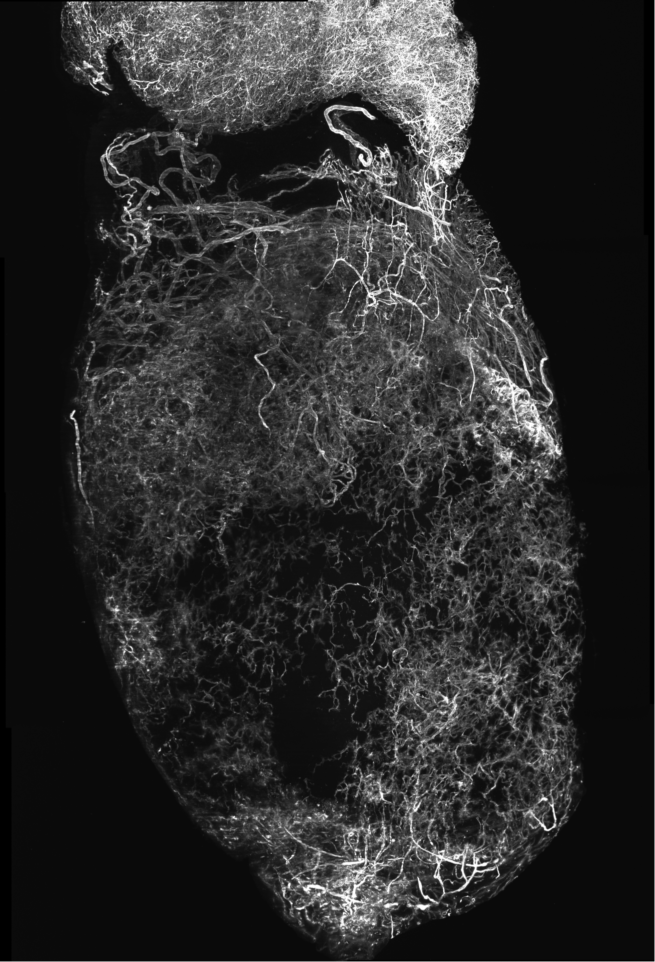
\includegraphics[scale=0.57]{fig/BloodVessels.png}
\end{figure}
%
%
\subsection{Prerequisites}
\label{sec:mod8prereq}
%
%

\begin{itemize}
\item 3D ImageJ Suite: To install the plugin select \ijmenu{Help > Update..}, click ''Manage Update Sites'', check ''3D ImageJ Suite'', click ''Close'' and then click ''Apply changes''.
For a description of the plugin see:\\
\url{http://imagejdocu.tudor.lu/doku.php?id=plugin:stacks:3d\_ij\_suite:start}.\\
We will use the multi-threaded 3D filters that can now be found in \ijmenu{Plugins > 3D > 3D Fast Filters} (you may have to restart ImageJ).\\

\item Look-up table with random colors: Please copy the file \textbf{"Random.lut"} into the ''luts'' folder of your ImageJ installation. We will use this LUT to visualize segmented objects in label images.

\item Restart ImageJ to make above actions come into effect.
\end{itemize}
%

%%%%%%%%%%%%%%%%%%%%%%%%%%%%%%%%%%%%%%%%%%%%%%%%%%%%%%%%%%
\section{Morphological closing of tubular structures}
%%%%%%%%%%%%%%%%%%%%%%%%%%%%%%%%%%%%%%%%%%%%%%%%%%%%%%%%%%
%
\subsection{Introduction}
As the overall aim of the project is to trace the blood vessel network, we are not interested in the tubes' hollow structure. In fact, for segmentation it would be easier if the tubes were plain, because then we would not have to deal with dark ''none-tube-voxels'' inside bright ''tube-voxels''. Our first task is thus to try to ''fill'' the tubes, using grayscale morphological closing (\cite{vincent1993morphological}.
%(see also section \ref{subsec:morphogray})).
%
\subsection{Workflow}
%
\begin{description}
%
\item[Data examination] \hfill \\ 
%
Open and view the data in Fiji using the following commands:

\item Open file: \ijmenu{File > Open...}  ''../bloodvessels\_small.tif''
\item View in 3D: \ijmenu{Plugins > 3D Viewer}
\item Change brightness (in 3D viewer menu): \ijmenu{[Edit > Transfer Function > RGBA]}
%
\item[Perform 3D morphological closing] \hfill \\ 
%
As the resolution of the dataset can be assumed reasonably isotropic and since the tubes can have any orientation we will use a spherical structuring element for the morphological closing. Select the CloseGray filter in \ijmenu{Plugins > 3D > 3D Fast Filters} with same kernel radius in all dimensions. A closing radius of 6 to 8 micrometers (3 to 4 voxels) is a sensible value for the dataset. This will not completely close the largest vessels however increasing the closing radius might merge the closest small vessels, so you have to go for a compromise here.  If you have time it is very instructive to also perform this grayscale closing operation by manually performing first a Maximum filter followed by Minimum filter.
%(see also section \ref{subsec:morphogray})).\\
%
\end{description}

\subsection{Generate an ImageJ macro}

Implement a macro performing above operations.

\underline{\textbf{Note}}: In the dialog box of the filters it is possible to input the radius in physical units or in pixels but only the radius in pixel shows up in the macro recorder. As it is convenient to input a radius in physical units you could write code to convert from micrometers to pixel units before calling the filter. For this you will require the macro function \ijmacro{getPixelSize}. In general, to combine numbers with the text strings as ImageJ plugin arguments you need \ijmacro{d2s(m,n)}, which converts a number m to a string keeping n decimals. 
%

%
\lstinputlisting{code/TubeAnalyst-1.ijm}
%
%

%%%%%%%%%%%%%%%%%%%%%%%%%%%%%%%%%%%%%%%%%%%%%%%%%%%%%%%%%%%%%%%
\section{Prefiltering to enhance filamentous voxels}
%%%%%%%%%%%%%%%%%%%%%%%%%%%%%%%%%%%%%%%%%%%%%%%%%%%%%%%%%%%%%%%
%
\subsection{Introduction}
The datasets used here exhibit a high contrast so that a simple intensity based thresholding is almost sufficient to distinguish tube from background voxels. However in case of higher noise and/or uneven sample staining one may need to filter the data prior to thresholding. A good criterion to follow for this operation is to notice that a voxel is part of a filament if there is one direction along which the intensity is quite constant (along the filament) and two perpendicular directions along which the intensities quickly drop (perpendicular to the filament). The ImageJ command \ijmenu{Plugins > Analyze > Tubeness} computes a metric reflecting to what extent a voxel and its local neighborhood fulfill this criterion. The implemented algorithm is based on \cite{Sato1998}. 
%
\subsection{Workflow}
%
Select the output image of above section (''Closed.tif'').
%
\begin{description}
%

\item[Enhance filamentous voxels]\hfill\\
%
Use the \ijmenu{Plugins > Analyze > Tubeness} command on the data (after the morphological closing) and check the result for different "Sigma", which controls the size of a Gaussian filter that is applied before the actual ''Tubeness'' computation.
%\ref{subsubsec:gaussian}) 
This Gaussian pre-filtering indirectly determines the size of the neighbourhood taken into account for computation of the local intensity distribution.

Sensible values are in the range of 6 to 8 micrometers but you can experiment with different values. It is in fact usually almost impossible to find a value that is optimal for both the smallest and the largest vessels. 

You will notice that the contrast is greatly enhanced after the filtering but voxels close to vessel branch points might be forced to zero as their neighborhood do not strictly follow the definition of being filamentous. If this problem is too pronounced it is possible to perform another pass of morphological closing after the pre-filtering to "repair" these gaps in the network.
\end{description}

\subsection{Generate an ImageJ macro script}
Implement a macro performing above operations.
%

\lstinputlisting{code/TubeAnalyst-2.ijm}
%
%%%%%%%%%%%%%%%%%%%%%%%%%%%%%%%%%%%%%%%%%%%%%%%%%%%%
\section{Segmentation of tubular structures}
%%%%%%%%%%%%%%%%%%%%%%%%%%%%%%%%%%%%%%%%%%%%%%%%%%%%
%
\subsection{Introduction}
In order to analyze the tubular network we need to decide whether a voxel is a part of a tube or part of the background. To do so we will threshold the data, i.e. assign voxels below or above a certain gray value as background or object. Typically such thresholding also yields spurious isolated voxels that are not part of the tubular network. We will clean up such voxels based on the criterion that they are rather isolated and not connected to many other voxels.
%
\subsection{Workflow}
%
\begin{description}
%
\item[Convert previous ("Tubeness") image to 8-bit]\hfill\\
This step is optional but it somewhat simplifies the following thresholding operation. You should be careful not to clip the intensities during the conversion: The easiest way is to find the voxel with minimum and maximum intensities in the stack by inspecting the stack histogram and setting the minimum and maximum intensity values of the display accordingly before the conversion with \ijmenu{Image > Adjust > Brightness/Contrast...} . 
%\ref{subsec:bitdepth}\\
%
\item[Generate a binary image]\hfill\\
%
Threshold the previous ("Tubeness") image using \ijmenu{Image > Adjust > Threshold} (manual, global thresholding). We recommend to convert the image to 8 bit before thresholding as the Adjust Threshold interface works better with 8 bit than with 32-bit format. The aim is to adjust the lower bound of the threshold so that most of the vessels are thresholded without getting merged (if you followed the previous 8-bit conversion step a lower bound intensity around 8 gray values should work fine for both datasets).
%

\textbf{\underline{Optional}}: Automated thresholding methods

If you have time you may explore some automated thresholding methods such as:
\begin{itemize}
\item \ijmenu{Image > Adjust > Auto Threshold}
\item \ijmenu{Image > Adjust > Auto Local Threshold}
\end{itemize}

\item[Clean up small objects] \hfill\\
Clean up object voxels that are isolated, i.e. not connected to a minimum number of neighboring object voxels. This can be done by using the "minimum volume" option of \ijmenu{Analyze > 3D Objects Counter}. You can compare the initial segmentation mask and the resulting label mask after running "3D Objects Counter" in order to see what objects have been discarded. A practical value for the minimum volume filter is around 1000 voxels but you can experiment with different values.
%

\textbf{\underline{Note}}: The voxels of the output have an intensity corresponding to the index of the connected object they are part of (label mask). The indexing starts at 1 and, depending on the active Look-Up Table (LUT), some objects can thus appear very faint. To better visualize the results it is handy to use the "Random.lut" (see section \ref{sec:mod8prereq}). Just select it from \ijmenu{Image > Lookup Tables} or call \ijmacro{run("Random")} from your macro script.

\end{description}

\subsection{Generate an ImageJ macro script}
Write a macro performing above operations. The lower bound of the threshold should be stored in a variable \textbf{VesselThreshold} and the minimum volume for each connected components should be called \textbf{VesselVolumeThreshold}.

\textbf{\underline{Note}}: For a proper 8-bit conversion of the Tubeness image you need to set the display to the minimum and maximum gray value of the image stack. In a macro the minimum and maximum value of the stack can be retrieved using \ijmacro{Stack.getStatistics(voxelCount, min, max, mean, std)} and the current bounds of the display can be set by \ijmacro{setMinAndMax(min, max)}.
%


\lstinputlisting{code/TubeAnalyst-3.ijm}

%%%%%%%%%%%%%%%%%%%%%%%%%%%%%%%%%%%%%%%%%%%%%%%%%%%%%%%%%%%%%%%%%%%%
\section{Skeletonization and analysis of the tubular network}
%%%%%%%%%%%%%%%%%%%%%%%%%%%%%%%%%%%%%%%%%%%%%%%%%%%%%%%%%%%%%%%%%%%%
%
\subsection{Introduction}
In order to measure the network length and to count its branch points we will reduce the segmented tubes (which have a certain thickness) to their 1 voxel wide center lines. This process is called "Skeletonization". 
%\ref{subsec:skelfilloutline}).
To identify the branch and end points of the skeletonized network one can use the following observations:
\begin{itemize}
\item End-point voxels have less than 2 neighbors.
\item Junction voxels have more than 2 neighbors.
\item Slab voxels (remaining voxels) have exactly 2 neighbors.
\end{itemize}
To perform these tasks we will use \ijmenu{Plugins > Skeleton > Skeletonize (2D/3D)} and \ijmenu{Plugins > Skeleton > Analyze Skeleton (2D/3D)} (see \cite{Arganda-Carreras2010}). Skeletonization is based on a specific connectivity. For 3D images ImageJ uses 26 neighbor per voxel by default.
%
\subsection{Workflow}

\begin{description}
%
\item[Skeletonization]\hfill\\
%
The label mask first needs to be binarized (all non zero voxels are objects) using \ijmenu{Image > Adjust > Threshold} with a lower threshold of 1 gray value. After this you can skeletonize the binary image using \ijmenu{Plugins > Skeleton > Skeletonize (2D/3D)}.  In order to visually check the skeletonization you may overlay the binary mask (or the original data) with the skeleton using for instance the command \ijmenu{Image > Color > Merge Channels...}. The original image might be assigned the gray channel and the skeleton the red channel.
%
\item[Skeleton analysis]\hfill\\
Use \ijmenu{Plugins > Skeleton > Analyze Skeleton (2D/3D)} to analyze the skeleton (for the moment leave all pruning options unchecked). Examine the image output, which has the following color-coding:
\begin{itemize}
\item End-point voxels: Gray value of 30, appearing blue.
\item Junction voxels: Gray value 70, appearing purple.
\item Slab voxels: Gray value 127, appearing red.
\end{itemize}
Examine the output table which not only contains the number of voxels falling into the three different classes but also the total length of the skeleton as well as their total number of end-points and junctions. If there are several disconnected skeletons in the image the statistics are reported for each of them. Observe that the number of junctions is smaller than the number of junction voxels, because at each junction there may be more than one voxel with more than two neighbors.
%
\item[Skeleton 3D visualization]\hfill\\
%
Visualize the analyzed skeleton in the 3D viewer. You may realize that it is not looking very nice, because it is only one voxel thick. Also the difference between slab, endpoint and branch voxels is not easy to see. 

\underline{Exercise}: Figure out a way to alter the skeleton for 3D visualization purposes.

\underline{Hint}: Change the value of the voxels by applying \ijmenu{Plugins > Process > Replace Value}; find an adequate combination of values and LUT, finally thicken the skeleton by dilating it in 3D. Be very careful when choosing the new values assigned to junction and end points as these voxels might be overwritten by close by slab voxels after dilation (local maximum operation).
\end{description}

\subsection{Generate an ImageJ macro script}
%
Implement a macro performing above operations.
%

\lstinputlisting{code/TubeAnalyst-4.ijm}

%%%%%%%%%%%%%%%%%%%%%%%%%%%%%%%%%%%%%%%%%%%%%%%%%%%%%%%%%%%%%%%%%%%%
\section{Skeleton pruning and holes closing (Optional)}
%%%%%%%%%%%%%%%%%%%%%%%%%%%%%%%%%%%%%%%%%%%%%%%%%%%%%%%%%%%%%%%%%%%%
%
\subsection{Introduction}
Depending on the roughness and thickness of the tubes in the raw data the computed skeleton may contain false positive short branches and/or false positive small loops. These can eventually be removed by a process called "pruning". We will test the different pruning algorithms implemented in \ijmenu{Plugins > Skeleton > Analyze Skeleton (2D/3D)}.
\subsection{Workflow}

\begin{description}
%
\item[End-point pruning]\hfill\\
%
Remove all branches containing exactly one end-point by checking the "Prune ends" option in \ijmenu{Plugins > Skeleton > Analyze Skeleton (2D/3D)}. Carefully examine the image and check whether the pruning is always working as you would expect (see also figure ~\ref{fig:prune}).
\begin{figure}[h!]
  \caption{Skeleton annotation and pruning. Slab voxels are white, junction voxels are red and end-point voxels are blue. Images are projections of 3D data and were subject to different processing steps: (Left) Skeletonization => Analysis. (Center Left) Skeletonization => Analysis with end-pruning. (Center Right) Skeletonization => Analysis with end-pruning => Analysis. (Right) Skeletonization => Analysis with end-pruning => Skeletonization => Analysis.} \label{fig:prune}
  \centering
    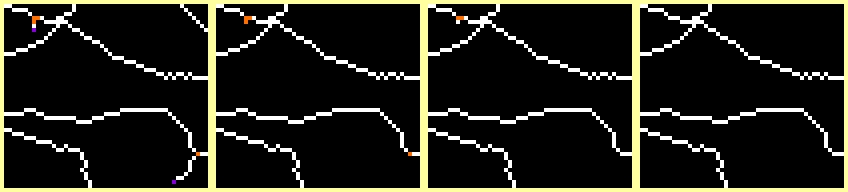
\includegraphics[width=1\textwidth]{fig/PruningStack--Montage.jpg}
\end{figure}
%
\item[Circular pruning]\hfill\\
%
Sometimes, especially when the cross-section of the tubes is large the skeletonization can lead to (small) false circular skeleton parts. If this is the case in your data try the "Prune cycle method" options of \ijmenu{Plugins > Skeleton > Analyze Skeleton (2D/3D)} and check if it  helped removing the false cycles.\\

\underline{Note}: One may consider additional algorithms; for instance to only remove branches up to a specified minimum length, however this is currently not implemented in \ijmenu{Analyze Skeleton (2D/3D)}. You should be very cautious with the pruning as important features of the network such as real loops and end point segments may also be removed. Using it or not boils down to a trade-off between removing spurious branches and removing real network branches. It is always better to try to obtain a good segmentation mask in the first place but, as you will notice, it is not easy to properly segment small and large vessels with such a simple image processing pipeline.

\item[Fill Holes]\hfill\\
The cycles in the large vessels usually originate from holes inside the segmented vessels, the problem can hence be mitigated by filling these holes in the binary mask before the skeletonization. This can be performed either in the 3D domain with \ijmenu{Plugins > 3D > 3D Fill Holes} or in 2D with \ijmenu{Process > Binary > Fill Holes}. In this last case we must specify in the command call that the operation should be applied to the whole stack (slice by slice). 

\underline{Note}:
More pixels will always be filled when the operation is performed in 2D, as a 2D hole appearing in a particular slice (e.g. a disk inside a cylinder) is not necessarily part of a 3D hole (the converse being true). In turn, 2D hole filling can generate some artifacts if the vessels form closed loops. 

\item[Morphological Closing] Sometimes the large vessels of the binary mask are not only hollow but a hole is pierced in their outside. These defects can lead to spurious small branches in the skeleton (as we saw before). If the holes are not too large they can be filled in by morphological closing of the binary mask. If you have time you can try this out.
%
\end{description}

\textbf{\underline{Note}}: The simple workflow proposed in this practical is working reasonably well on the datasets we acquired, but, as we saw, it is pretty limited when it comes to segment a mixture of thin and thick vessels in the same stack. It cannot compete with some high accuracy filament tracing methods, some of which are reviewed in \cite{lesage2009review}. More specifically, a very clever method is described in \cite{li2006vessels}. 

%\lstinputlisting{code/TubeAnalyst-5.ijm}

%%
%%%%%%%%%%%%%%%%%%%%%%%%%%%%%%%%%%%%%%%%%%%%%%%%%%%%%%%%%%%%%%%%%%%%
\section{Extraction of biologically relevant parameters}
%%%%%%%%%%%%%%%%%%%%%%%%%%%%%%%%%%%%%%%%%%%%%%%%%%%%%%%%%%%%%%%%%%%%
%
\subsection{Introduction}
As was previously motivated in section \ref{sec:mod8lab0} the density of the vascularization and branching points and the thickness of the vessels are crucial age indicators to understand how a tumour developed and possibly necrosed. We will now estimate these parameters on the segmented data.
%
\subsection{Workflow}
%
\begin{description}
%
\item[Generate an ImageJ macro script]\hfill\\
The computation of the biologically relevant parameters cannot be achieved via the ImageJ menu, but you have to write an ImageJ macro.
%
\item[Vessel length and number of branch points]\hfill\\
%
To compute the total vessel length you have to loop through the entries of the results table that you got from \ijmenu{Plugins > Skeleton > Analyze Skeleton (2D/3D)} and add up and/or multiply the respective entries in the respective columns (''\# Branches'', ''Average Branch Length''). In addition to for-looping through the rows of the results table, you will need the \ijmacro{getResult("Column", row)} macro function in order to extract the values from the table.
%
\item[Vessel volume and total imaged volume]\hfill\\
%
To compute the total vessel volume you should use the information obtained from the ImageJ macro function \ijmacro{Stack.getstatistics}. The volume can be expressed in voxel units or in physical unit. For the conversion the calibration can be retrieved with \ijmacro{getPixelSize(width, height, depth, unit)}.

\item[Density of vascularization]\hfill\\
To derive the density of vascularization one needs to compute the fraction of space occupied by the vessels. This can be done by dividing the volume previously computed by the total imaged volume, which you can compute using a combination of the following functions:
\begin{itemize}
\item \ijmacro{getWidth()}
\item \ijmacro{getHeight()}
\item \ijmacro{nSlices}
\end{itemize}
%
\item[Vessel width]\hfill\\
The average vessel width can readily be computed from the parameters we previously extracted... can you figure out how?

\end{description}

\subsection{Generate an ImageJ macro script}

Implement a macro perfroming the above operations.

\textbf{\underline{Hint}}: The easiest way is to estimate the average section of the vessels and then only to derive their average thickness by assuming their section is close to a disk.
%


\lstinputlisting{code/TubeAnalyst-6.ijm}

%%%%%%%%%%%%%%%%%%%%%%%%%%%%%%%%%%%%%%%%%%%%%%%%%%%%%%%%%%%%%%%%%%%%
\section{Graphical user interface (GUI)}
\label{sec:mod8lab1}
%%%%%%%%%%%%%%%%%%%%%%%%%%%%%%%%%%%%%%%%%%%%%%%%%%%%%%%%%%%%%%%%%%%%
%
The pipeline of operations we came up with can now be assembled to a complete macro to process the original stacks. Here, we add a dialog box allowing the user to enter the macro parameters via a GUI. The GUI can be created using the following macro commands:
\begin{itemize}
\item \ijmacro{Dialog.create}
\item \ijmacro{Dialog.addNumber}
\item \ijmacro{Dialog.show}
\item \ijmacro{Dialog.getNumber}
\end{itemize}
Add the dialog box to the beginning of your macro code and make sure that the names of the parameters (variables) that you retrieve from the GUI are the same as the parameters in your macro code. In addition you have to remove (comment out) the explicit assignments of the input parameters from your macro code (otherwise these explicit assignments will overwrite the assignments from the GUI).   

\lstinputlisting{code/TubeAnalyst-7.ijm}

%%%%%%%%%%%%%%%%%%%%%%%%%%%%%%%%%%%%%%%%%%%%%%%%%%%%%%%%%%%%%%%%%%%%
\section{3-D results visualization}
%%%%%%%%%%%%%%%%%%%%%%%%%%%%%%%%%%%%%%%%%%%%%%%%%%%%%%%%%%%%%%%%%%%%
%
At the end of the macro we can automatically load, show and even animate the data in the 3-D viewer, using commands such as:
\begin{itemize}
\item \ijmacro{run("3D Viewer");}
\item \ijmacro{call("ij3d.ImageJ3DViewer.setCoordinateSystem", "false");}
\item \ijmacro{call("ij3d.ImageJ3DViewer.add", "ImageName", "None", "RefToImageName", "0", "true", "true", "true", "2", "0");}
\item \ijmacro{call("ij3d.ImageJ3DViewer.startAnimate");}
\item \ijmacro{wait(NumberOfMilliseconds);}
\item \ijmacro{call("ij3d.ImageJ3DViewer.stopAnimate");}
\end{itemize}
The third item is used to add an image called "ImageName" to the viewer and label it "RefToImageName" in the 3D viewer \ijmenu{Edit > Select ..} menu entry.
%
In case you did not have time to write up the complete macro during the practical a possible solution is provided in: (code/\textbf{TubeAnalyst.ijm}). An example overlay of the output files is shown in figure ~\ref{fig:bloodvesselsproj}.

\begin{figure}
  \caption{Maximum intensity projection of the original dataset with overlaid skeleton} 
  \label{fig:bloodvesselsproj}
  \centering
    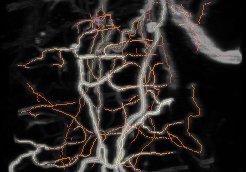
\includegraphics[scale=1]{fig/Projection.png}
\end{figure}

\lstinputlisting{code/TubeAnalyst-8.ijm}

%%%%%%%%%%%%%%%%%%%%%%%%%%%%%%%%%%%%%%%%%%%%%%%%%%%%
\section{Assignments}
%%%%%%%%%%%%%%%%%%%%%%%%%%%%%%%%%%%%%%%%%%%%%%%%%%%%
%
\begin{description}
%
\item[3D viewer automation] \hfill \\
Add some more 3D viewer macro controls (in the last part of the complete macro). It is for instance possible to control the transparency of each object and many more features of the 3D viewer. You can experiment with it by recording these actions. Try to be creative!
%
\item[Local statistics] \hfill \\
Write a macro to split the original stack in several sub-volumes of user defined size and estimate all the previous geometrical parameters in each of the sub-volumes. Doing so, one can access to the local values of these biological parameters. For this assignment you should rather use the larger stack (you might first need to slightly tune the parameters of your work-flow to get a valid segmentation). It is possible to run the whole pipeline on each sub-volume or, more efficiently, to run it once on the whole stack up to the segmentation and extract the information of interest in each sub-volume afterwards. 
%
\end{description}

%%%%%%%%%%%%%%%%%%%%%%%%%%%%%%%%%%%%%%%%%%%%%%%%%%%%
%\section{Complete ImageJ Macro}
%\label{sec:mod8lab2}
%%%%%%%%%%%%%%%%%%%%%%%%%%%%%%%%%%%%%%%%%%%%%%%%%%%%
%
%\lstinputlisting{code/TubeAnalyst_v5.ijm}
%
\section{Acknowledgements}
We would like to thank Alexandre Calon (IRB Barcelona) for preparing the mice and helping us set up the foundations of tumors quantitative analysis from MacroSPIM images.
\bibliographystyle{plainnat}
\bibliography{module8references}

\end{document}
